\documentclass[11pt]{article}
\usepackage[utf8]{inputenc}
\usepackage[T1]{fontenc}
\usepackage[margin=2cm]{geometry}
\usepackage{tikz}
\usepackage{tcolorbox}
\usepackage{array}
\usepackage{amsmath}
\usepackage{amssymb}
\usepackage{graphicx}
\usepackage{fancyhdr}
\usepackage{enumitem}

\tcbuselibrary{skins}
\pagestyle{empty}

% ---- En-tête Nom / Groupe ----
\newcommand{\entete}{%
  \noindent Nom: \rule{6.5cm}{0.4pt} \hfill Groupe: \rule{3cm}{0.4pt}\\[4mm]
}

% ---- Boîte "Cible" avec titre en gras dans la boîte ----
\newtcolorbox{cible}[1]{
  colback=white, colframe=black, boxrule=0.6pt, arc=0pt,
  left=4mm, right=4mm, top=2mm, bottom=2mm,
  fonttitle=\bfseries, coltitle=black,
  before upper={\textbf{#1}\par\smallskip}
}

% ---- Case blanche générique (pour les chaînes d'opérations) ----
\newcommand{\caseop}[1]{%
  \begin{minipage}[t][3cm][t]{\linewidth}
  #1
  \end{minipage}
}

\begin{document}

%==================== PAGE 1 ====================
\entete
\noindent \textbf{Évaluation: Exposants et chaînes d'opérations} \hfill Chapitre 1
\vspace{2mm}
\hrule
\vspace{4mm}

\begin{cible}{Cible 1: Représenter, écrire et calculer des nombres en notation exponentielle.}

1. Trouve les puissances suivantes.
\vspace{2mm}

\begin{tabular}{@{}p{0.5cm}p{2.3cm}p{4.3cm}p{0.5cm}p{2.3cm}p{4.3cm}@{}}
a) & $2^3 = $ & \rule{3.2cm}{0.4pt} & b) & $4^2 = $ & \rule{3.2cm}{0.4pt} \\[4mm]
c) & $9^0 = $ & \rule{3.2cm}{0.4pt} & d) & $8^1 = $ & \rule{3.2cm}{0.4pt} \\[4mm]
e) & $(-3)^2 = $ & \rule{3.2cm}{0.4pt} & f) & $(-5)^3 = $ & \rule{3.2cm}{0.4pt} \\[4mm]
g) & $-(5^2) = $ & \rule{3.2cm}{0.4pt} & h) & $-4^2 = $ & \rule{3.2cm}{0.4pt} \\
\end{tabular}

\vspace{6mm}
\noindent 2. Factorise 28 en nombres premiers.

\vspace{2.5cm}

\noindent Rép: $28 = $ \rule{3.5cm}{0.4pt}


\vspace{6mm}
\noindent 3. Factorise 315 en nombres premiers.

\vspace{2.5cm}

\noindent Rép: $315 = $ \rule{3.5cm}{0.4pt}

\vspace{6mm}

\noindent 4. Factorise 297 en nombres premiers.

\vspace{2.5cm}

\noindent Rép: $297 = $ \rule{3.5cm}{0.4pt}
\vspace{4mm}
\end{cible}

\vfill
\begin{center}
1
\end{center}

\newpage

%==================== PAGE 2 ====================
\entete

\begin{cible}{Cible 2: Situer et comparer des nombres entiers.}

1. Compare les expressions suivantes à l'aide des symboles $<, >$ et $=$. 

\vspace{1cm}

\textbf{CALCULS OBLIGATOIRES}

\vspace{1cm}

\begin{tabular}{|p{7.7cm}|p{7.7cm}|}
\hline
\rule{0pt}{4mm} a) $4^2 \; \underline{\hspace{1cm}} \; 2^4$ & d) $-3^2 \; \underline{\hspace{1cm}} \; (-3)^2$ \\[3.2cm]
\hline
\rule{0pt}{4mm} e) $-8 \times 11 \; \underline{\hspace{1cm}} \; 3^3 \times -11$ & f) $\quad 4 \times 6 - (-4)^3 = $ \\[3.2cm]
\hline
\end{tabular}

\vspace{2mm}
\begin{tabular}{@{}p{0.5cm}p{5.5cm}@{}p{0.5cm}p{5.5cm}@{}p{0.5cm}p{4cm}@{}}
& $4^2 \; \underline{\hspace{1cm}} \; 2^4$ &  & $-3^2 \; \underline{\hspace{1cm}} \; (-3)^2$ \\[4mm]
& $-8 \times 11 \; \underline{\hspace{1cm}} \; 3^3 \times -11$ & e) & $-40 + 20 \; \underline{\hspace{1cm}} \; -7 \times 3$ \\

\end{tabular}


\vspace{6mm}
\noindent 2. Parmi les valeurs suivantes, laquelle est la plus grande? Encercle la bonne réponse.

\vspace{2mm}
\begin{tabular}{@{}p{0.5cm}p{3cm}p{0.5cm}p{3.5cm}p{0.5cm}p{3cm}p{0.5cm}p{3cm}@{}}
a) & $-3^2$ & b) & L'opposé de 15 & c) & $-6 + 3^2$ & d) & $(8-12)^2$ \\
\end{tabular}

\end{cible}

\vspace{5mm}

\begin{cible}{Cible 3: Effectuer des chaînes d'opérations.}

1. Trouve le résultat en utilisant la méthode de l'entonnoir.

\vspace{2mm}
\renewcommand{\arraystretch}{1}
\begin{tabular}{|p{7.7cm}|p{7.7cm}|}
\hline
a) $\quad 6 \times (4+3) = $ & b) $\quad 7 - (-6)^2 = $ \\[3.2cm]
\hline
\end{tabular}

\end{cible}

\vfill
\begin{center}
2
\end{center}

\newpage

%==================== PAGE 3 ====================
\entete

\renewcommand{\arraystretch}{1}
\begin{tabular}{|p{7.7cm}|p{7.7cm}|}
\hline
\rule{0pt}{4mm} c) $\quad (-2)^3 - 7 = $ & d) $\quad 5 \times -9 + 4 = $ \\[3.2cm]
\hline
\rule{0pt}{4mm} e) $\quad 5 \times 9 - 50 \div (12-2) = $ & f) $\quad 4 \times 6 - (-4)^3 = $ \\[3.2cm]
\hline
\rule{0pt}{4mm} g) $\quad (-7+5)^3 \div 4 = $ & h) $\quad (-7)^2 - 8 + 4 \div -4 = $ \\[3.2cm]
\hline
\end{tabular}

\vfill
\begin{center}
3
\end{center}

\newpage

%==================== PAGE 4 ====================
\entete

\noindent Problème en contexte (\textbf{montre ta démarche et tes calculs})

\vspace{3mm}
\begin{minipage}[t]{0.62\linewidth}
Sophie et Laurence jouent une partie de dards. Elles lancent chacune 25 fléchettes.

\vspace{2mm}
Sophie a atteint 12 fois l'anneau de 10 points, 9 fois l'anneau de -15 points, 3 fois l'anneau de -20 points et une seule fois le centre de 25 points.

\vspace{2mm}
Laurence a atteint 9 fois l'anneau de 10 points, 11 fois l'anneau de -15 points, 2 fois la zone de -20 points et 3 fois la zone de 25 points.

\vspace{2mm}
Sophie croit qu'elle obtient un plus grand nombre de points et donc, qu'elle gagne la partie contre Laurence.

\vspace{2mm}
A-t-elle raison? Explique.
\end{minipage}%
\hfill
\begin{minipage}[t]{0.34\linewidth}
\centering
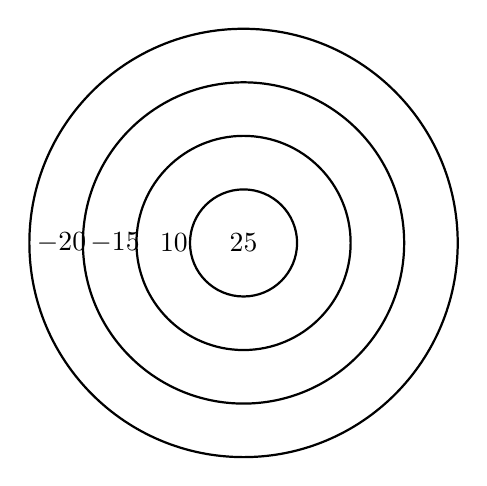
\begin{tikzpicture}[scale=0.68, baseline=(current bounding box.north)]
  \draw[thick] (0,0) circle (4);
  \draw[thick] (0,0) circle (3);
  \draw[thick] (0,0) circle (2);
  \draw[thick] (0,0) circle (1);
  \node at (-3.4,0) {$-20$};
  \node at (-2.4,0) {$-15$};
  \node at (-1.3,0) {$10$};
  \node at (0,0) {$25$};
\end{tikzpicture}
\end{minipage}

\vfill
\begin{center}
4
\end{center}

\end{document}